\documentclass[aspectratio=169,10pt]{beamer}

\usetheme{metropolis}
\usepackage{appendixnumberbeamer}
\usepackage{booktabs}
\usepackage[scale=2]{ccicons}
\usepackage{pgfplots}
\usepgfplotslibrary{dateplot}
\usepackage{xspace}
\usepackage{tikz}
\usetikzlibrary{mindmap,trees,shapes,arrows,positioning,pie}
\usepackage{tcolorbox}
\usepackage{fontawesome5}

\newcommand{\themename}{\textbf{\textsc{metropolis}}\xspace}

\title{Understanding the PhD Landscape in Europe and Germany}
\subtitle{Session 2: Funding, Practical Considerations, and Challenges}
\date{\today}
\author{Dr. Bijun Li}
\institute{Max Planck Institute for Meteorology}

\begin{document}

\maketitle

\begin{frame}{Recap and Today's Agenda}
\begin{columns}[T]
    \begin{column}{0.5\textwidth}
        \alert{Recap from Talk 1}
        \begin{itemize}
            \item European PhD landscape diversity
            \item German higher education system
            \item Finding opportunities
            \item Application process
        \end{itemize}
    \end{column}
    \begin{column}{0.5\textwidth}
        \alert{Today's Agenda}
        \begin{itemize}
            \item Funding sources and financial planning
            \item Practical considerations for PhD life
            \item Overcoming common challenges
            \item Building your professional network
            \item Career development strategies
        \end{itemize}
    \end{column}
\end{columns}

\vspace{0.5cm}
\centering
\tikz\node[draw,rounded corners,fill=blue!20,text width=0.8\textwidth]{
    Our goal: Equip you with practical knowledge and strategies for a successful PhD journey in Germany
};
\end{frame}

\begin{frame}{Learning Objectives for Today}
    By the end of this session, you will be able to:
    \begin{itemize}
        \item Identify and evaluate various funding sources for your PhD
        \item Create a realistic budget for living in Germany as a PhD student
        \item Understand and prepare for common challenges in PhD life
        \item Develop strategies for work-life balance and cultural integration
        \item Start building a professional network in your field
        \item Explore potential career paths after your PhD
    \end{itemize}
\end{frame}

\begin{frame}{Overview of Funding Sources}
\begin{columns}[T]
    \begin{column}{0.5\textwidth}
        \begin{itemize}
            \item Government Grants: DAAD, DFG
            \item EU Funding: MSCA, Erasmus+, ERC
            \item University Funding: Positions, Scholarships
            \item Industry Partnerships
            \item External Programs: Foundations, NGOs
        \end{itemize}
    \end{column}
    \begin{column}{0.5\textwidth}
        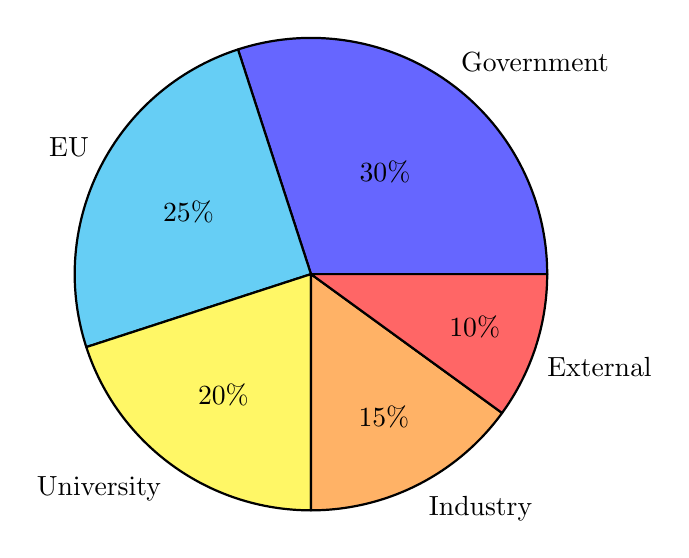
\begin{tikzpicture}
            \pie{30/Government, 25/EU, 20/University, 15/Industry, 10/External}
        \end{tikzpicture}
    \end{column}
\end{columns}

\vspace{0.3cm}
\alert{Success Rates and Application Tips}
\begin{itemize}
    \item DAAD: \textasciitilde20% success rate. Tip: Focus on your motivation and future plans.
    \item DFG: \textasciitilde30% success rate. Tip: Emphasize the innovative aspects of your research.
    \item MSCA: \textasciitilde12% success rate. Tip: Highlight the European dimension of your project.
\end{itemize}

\alert{Combining Funding Sources}
\begin{itemize}
    \item Example: 65% university position + 35% industry partnership
    \item Caution: Check regulations on additional income
\end{itemize}
\end{frame}

\begin{frame}{Financial Aspects of PhD Life}
\begin{columns}[T]
    \begin{column}{0.5\textwidth}
        \alert{Monthly Expenses (Estimated)}
        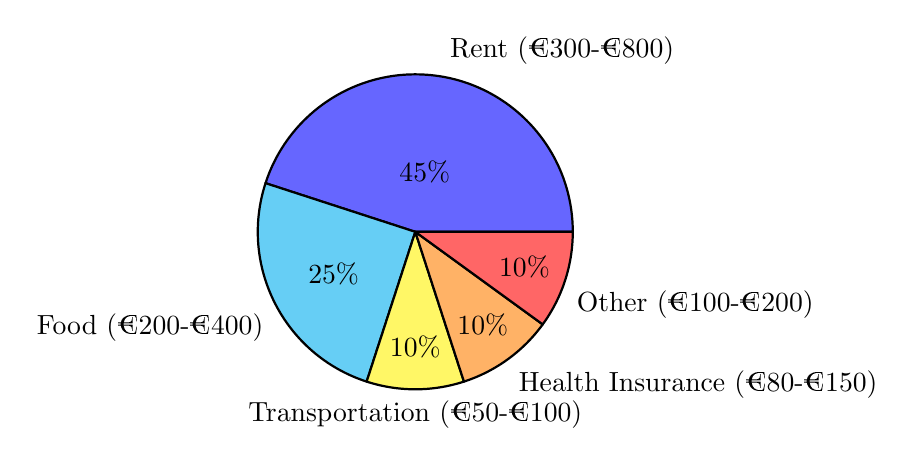
\begin{tikzpicture}
            \pie[radius=2]{
                45/Rent (€300-€800),
                25/Food (€200-€400),
                10/Transportation (€50-€100),
                10/Health Insurance (€80-€150),
                10/Other (€100-€200)
            }
        \end{tikzpicture}
    \end{column}
    \begin{column}{0.5\textwidth}
        \alert{Cost Comparison (Monthly)}
        \begin{tabular}{|l|c|c|}
        \hline
        Expense & Munich & Leipzig \\
        \hline
        Rent & €700 & €400 \\
        Food & €300 & €250 \\
        Transport & €70 & €50 \\
        \hline
        \end{tabular}
    \end{column}
\end{columns}

\vspace{0.3cm}
\alert{Tax Implications}
\begin{itemize}
    \item PhD positions: Taxed as regular income
    \item Scholarships: Often tax-free, but check specific terms
    \item Tax returns: Can often result in refunds
\end{itemize}

\alert{Budgeting Tools}
\begin{itemize}
    \item DAAD Cost of Living Calculator: \url{www.daad.de/deutschland/nach-deutschland/voraussetzungen/en/9198-financing/}
    \item Numbeo: \url{www.numbeo.com/cost-of-living/}
    \item Mobile apps: Mint, YNAB (You Need A Budget)
\end{itemize}
\end{frame}

\begin{frame}{Practical Considerations for PhD Students in Germany}
    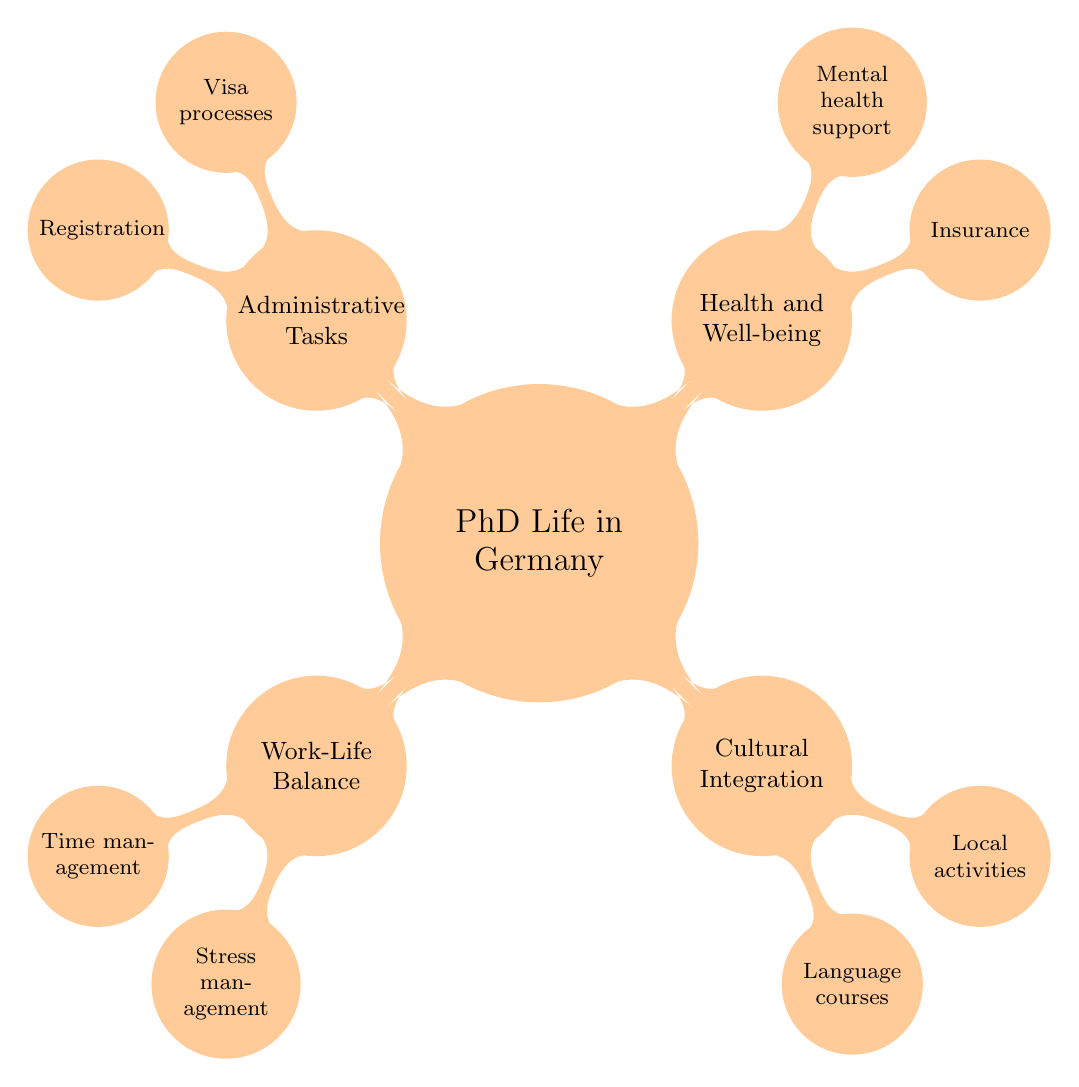
\begin{tikzpicture}[mindmap, grow cyclic, every node/.style=concept, concept color=orange!40, 
                        level 1/.append style={level distance=4cm,sibling angle=90},
                        level 2/.append style={level distance=3cm,sibling angle=45}]
        
        \node{PhD Life in Germany}
        child { node {Work-Life Balance}
            child { node {Time management} }
            child { node {Stress management} }
        }
        child { node {Cultural Integration}
            child { node {Language courses} }
            child { node {Local activities} }
        }
        child { node {Health and Well-being}
            child { node {Insurance} }
            child { node {Mental health support} }
        }
        child { node {Administrative Tasks}
            child { node {Visa processes} }
            child { node {Registration} }
        };
    \end{tikzpicture}
\end{frame}

\begin{frame}{Housing Options in Germany}
\alert{Types of Accommodation}
\begin{itemize}
    \item Student dormitories (Studentenwohnheim): €200-€400/month
    \item Shared apartments (WG - Wohngemeinschaft): €300-€600/month
    \item Private apartments (Einzelapartment): €400-€1000+/month
\end{itemize}

\alert{Finding Accommodation}
\begin{itemize}
    \item University housing offices: Often have reserved spots for international students
    \item Websites: WG-Gesucht.de, Immobilienscout24.de, eBay Kleinanzeigen
    \item Facebook groups: "Wohnungen in [City Name]" or "[City Name] Housing"
    \item Local newspapers and bulletin boards
\end{itemize}

\alert{Tips for Apartment Hunting}
\begin{itemize}
    \item Start early (at least 2-3 months before arrival)
    \item Prepare necessary documents (proof of income, Schufa, copy of passport)
    \item Be aware of additional costs (Nebenkosten): Usually 15-20% of base rent
    \item Consider temporary accommodation for your first weeks (e.g., Airbnb, hostels)
    \item Understand rental terms: "kalt" (excluding utilities) vs. "warm" (including utilities)
    \item Be cautious of scams: Never transfer money before seeing the apartment and signing a contract
\end{itemize}
\end{frame}

\begin{frame}{Navigating German Bureaucracy}
\alert{Key Administrative Tasks}
\begin{itemize}
    \item City Registration (Anmeldung): Required within 2 weeks of arrival
    \item Residence Permit (Aufenthaltserlaubnis): Apply within 90 days of arrival
    \item Health Insurance: Mandatory for all students
    \item Opening a Bank Account: Essential for rent and salary payments
\end{itemize}

\alert{Useful Resources}
\begin{itemize}
    \item University International Office: Your first point of contact
    \item City's Foreigners' Office (Ausländerbehörde): For visa and residence matters
    \item EURAXESS Services Centre: Supports international researchers
    \item Make it in Germany: Official portal for international qualified professionals
\end{itemize}

\alert{Tips for Smooth Process}
\begin{itemize}
    \item Start paperwork early: Some processes can take several weeks
    \item Keep multiple copies of all important documents
    \item Consider using a translation service for official documents
    \item Don't hesitate to ask for help from your university or colleagues
    \item Learn basic German phrases for bureaucratic processes
    \item Be patient and polite: Bureaucracy can be frustrating, but stay calm
\end{itemize}
\end{frame}

\begin{frame}{Overcoming Challenges in Your PhD Journey}
\begin{columns}[T]
    \begin{column}{0.5\textwidth}
        \alert{Common Challenges}
        \begin{itemize}
            \item Imposter syndrome
            \item Work-life balance
            \item Supervisor conflicts
            \item Research setbacks
            \item Cultural adaptation
            \item Language barriers
        \end{itemize}
    \end{column}
    \begin{column}{0.5\textwidth}
        \alert{Coping Strategies}
        \begin{itemize}
            \item Peer support groups
            \item Time management techniques (e.g., Pomodoro)
            \item Regular communication with supervisor
            \item Mindfulness and stress-reduction practices
            \item Language tandem partnerships
            \item Seeking professional help when needed
        \end{itemize}
    \end{column}
\end{columns}

\vspace{0.3cm}
\alert{Case Study: Overcoming Imposter Syndrome}
\begin{tcolorbox}[colback=green!5,colframe=green!40!black]
Maria, a PhD student from Spain, initially felt overwhelmed by the expertise of her peers. She joined a peer support group, practiced positive self-talk, and focused on her unique contributions. Over time, she gained confidence and even mentored new students.
\end{tcolorbox}

\alert{Additional Resources}
\begin{itemize}
    \item "The PhD Survival Guide" by Andres Ruiz
    \item "The Unwritten Rules of PhD Research" by Marian Petre and Gordon Rugg
    \item Online communities: Reddit r/PhD, The Grad Cafe
\end{itemize}
\end{frame}

\begin{frame}{Mental Health Resources for PhD Students in Germany}
\alert{University Services}
\begin{itemize}
    \item Psychological counseling centers (Psychologische Beratungsstelle)
    \item Graduate school support programs
    \item Workshops on stress management and work-life balance
    \item Peer mentoring programs
\end{itemize}

\alert{External Resources}
\begin{itemize}
    \item TelefonSeelsorge: 0800 111 0 111 (24/7 hotline, in German)
    \item International Student Helpline: +49 30 20177857
    \item Mind: The Mental Health Charity (online resources in English)
    \item Nightline: Student-run listening services in various German cities
\end{itemize}

\alert{Self-Help Strategies}
\begin{itemize}
    \item Regular exercise and healthy diet
    \item Mindfulness and meditation apps (e.g., Headspace, Calm)
    \item Maintaining social connections
    \item Setting realistic goals and celebrating small wins
    \item Time management techniques (e.g., Eisenhower Matrix)
    \item Hobbies and activities outside of research
\end{itemize}

\alert{When to Seek Professional Help}
\begin{itemize}
    \item Persistent feelings of sadness or anxiety
    \item Significant changes in sleep or eating patterns
    \item Difficulty concentrating or making decisions
    \item Thoughts of self-harm or suicide
\end{itemize}
\end{frame}

\begin{frame}{Building Your Professional Network}
\begin{columns}[T]
    \begin{column}{0.6\textwidth}
        \alert{Networking Opportunities}
        \begin{itemize}
            \item Academic conferences (e.g., ECPR General Conference)
            \item Summer schools (e.g., Essex Summer School in Social Science Data Analysis)
            \item Professional societies (e.g., German Physical Society)
            \item University seminars and workshops
            \item Online platforms (ResearchGate, Academia.edu)
            \item Social media (Twitter, LinkedIn)
            \item Interdisciplinary events (e.g., Science Slams)
        \end{itemize}
    \end{column}
    \begin{column}{0.4\textwidth}
        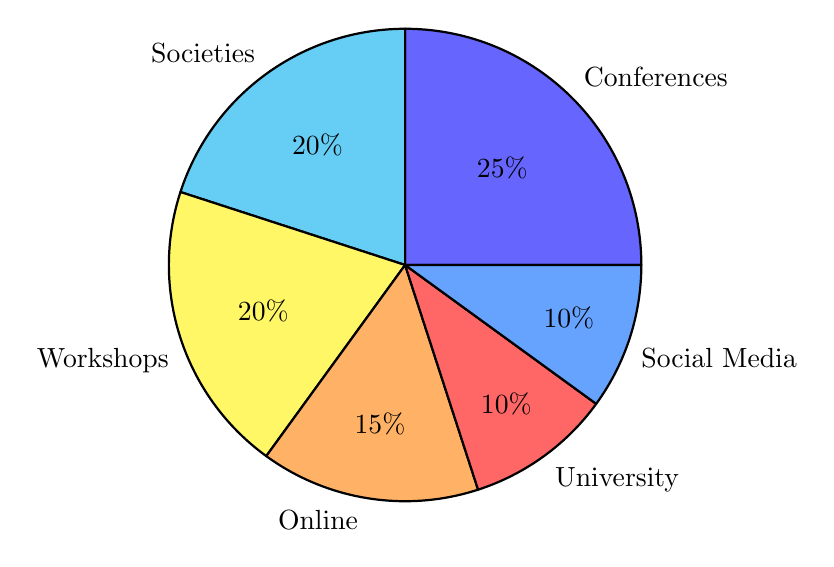
\begin{tikzpicture}
            \pie{25/Conferences, 20/Societies, 20/Workshops, 15/Online, 10/University, 10/Social Media}
        \end{tikzpicture}
    \end{column}
\end{columns}

\vspace{0.3cm}
\alert{Networking Tips}
\begin{itemize}
    \item Prepare an "elevator pitch" about your research
    \item Follow up with new contacts within a week
    \item Offer help or resources to others in your network
    \item Engage regularly on professional social media platforms
    \item Consider starting a blog or podcast about your research area
    \item Volunteer at conferences or local scientific events
    \item Join or create a journal club in your field
\end{itemize}

\alert{Cultural Considerations in German Academic Networking}
\begin{itemize}
    \item Formal address: Use titles (e.g., "Prof. Dr.") unless invited to use first names
    \item Punctuality: Being on time is highly valued in German culture
    \item Direct communication: Germans often appreciate straightforward, honest discussions
\end{itemize}
\end{frame}

\begin{frame}{Maximizing Your Professional Development}
\alert{Key Skills to Develop}
\begin{itemize}
    \item Academic writing and publishing
    \item Grant writing and proposal development
    \item Project management and time management
    \item Data analysis and visualization
    \item Teaching and mentoring
    \item Science communication and public speaking
    \item Collaboration and teamwork
    \item Leadership and lab management
\end{itemize}

\alert{Professional Development Opportunities in Germany}
\begin{itemize}
    \item Graduate school workshops and seminars
    \item DAAD STIBET Doktoranden program
    \item Coursera and edX online courses
    \item Language courses at university language centers
    \item Industry internships (check your contract regulations)
    \item Teaching assistantships
    \item Organizing conferences or workshops
\end{itemize}

\alert{Building Your Personal Brand}
\begin{itemize}
    \item Create a professional website or blog
    \item Maintain an up-to-date ORCID profile
    \item Engage in science communication (e.g., "Pint of Science" events)
    \item Contribute to open-source projects in your field
    \item Develop a consistent online presence across platforms
    \item Consider creating video content (e.g., YouTube tutorials in your field)
\end{itemize}

\alert{Tracking Your Progress}
\begin{itemize}
    \item Keep a skills development journal
    \item Set SMART goals for each semester
    \item Regularly update your CV and research statement
    \item Seek feedback from mentors and peers
\end{itemize}
\end{frame}

\begin{frame}{Career Paths After Your PhD}
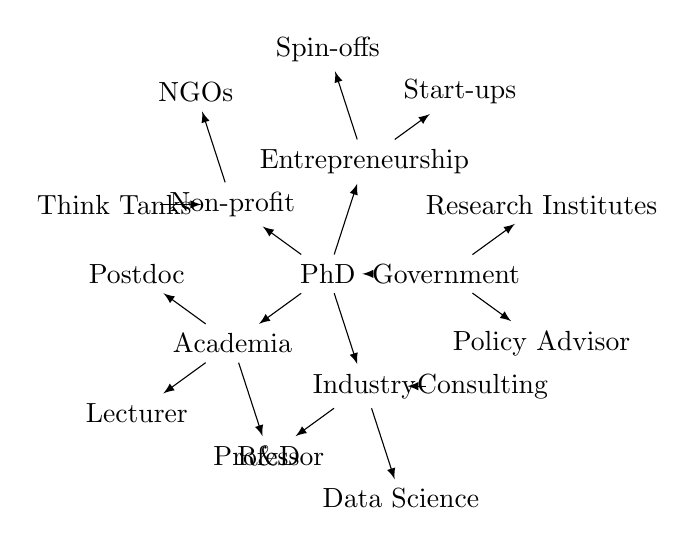
\begin{tikzpicture}[grow cyclic, ->,>=latex, level 1/.style={sibling angle=72}]
\node[](z){PhD}
  child{node[]{Academia}
    child{node[]{Postdoc}}
    child{node[]{Lecturer}}
    child{node[]{Professor}}}
  child{node[]{Industry}
    child{node[]{R\&D}}
    child{node[]{Data Science}}
    child{node[]{Consulting}}}
  child{node[]{Government}
    child{node[]{Policy Advisor}}
    child{node[]{Research Institutes}}}
  child{node[]{Entrepreneurship}
    child{node[]{Start-ups}}
    child{node[]{Spin-offs}}}
  child{node[]{Non-profit}
    child{node[]{NGOs}}
    child{node[]{Think Tanks}}};
\end{tikzpicture}

\vspace{0.3cm}
\alert{German Job Market for PhD Holders}
\begin{itemize}
    \item Strong demand in STEM fields, particularly in industry
    \item Growing opportunities in data science and AI across sectors
    \item Increasing recognition of PhD skills in non-academic sectors
    \item Emerging roles in sustainability and renewable energy
    \item Opportunities in Germany's Mittelstand (small and medium-sized enterprises)
\end{itemize}

\alert{Career Planning Tips}
\begin{itemize}
    \item Start exploring options early in your PhD (by year 2)
    \item Gain transferable skills through workshops and side projects
    \item Network with professionals in various sectors
    \item Consider doing an internship or collaborative project with industry
    \item Attend career fairs and alumni events
    \item Explore the German job market through platforms like Xing and StepStone
\end{itemize}
\end{frame}

\begin{frame}{Work Culture in German Academia}
\alert{Key Characteristics}
\begin{itemize}
    \item Hierarchical structure with clear roles and responsibilities
    \item Strong emphasis on formal qualifications and titles
    \item High value placed on punctuality and efficiency
    \item Direct communication style
    \item Work-life balance is generally respected
\end{itemize}

\alert{Academic Traditions}
\begin{itemize}
    \item Habilitation: Post-doctoral qualification for professorship
    \item Academic freedoms: "Freiheit von Forschung und Lehre"
    \item Emphasis on theoretical foundations and methodological rigor
\end{itemize}

\alert{Tips for International PhD Students}
\begin{itemize}
    \item Learn and use proper forms of address (e.g., "Herr Professor" or "Frau Doktor")
    \item Be prepared for direct feedback and criticism
    \item Respect work hours and vacation time
    \item Engage in departmental activities and traditions
    \item Take advantage of interdisciplinary collaboration opportunities
\end{itemize}
\end{frame}

\begin{frame}{Publishing and Conferences during Your PhD}
\alert{Publishing Strategies}
\begin{itemize}
    \item Aim for a mix of journal articles and conference papers
    \item Consider open access options (check university policies)
    \item Start with smaller conference papers to build confidence
    \item Collaborate on papers with peers and advisors
    \item Be aware of predatory journals and conferences
\end{itemize}

\alert{Conference Participation}
\begin{itemize}
    \item Attend both international and German conferences
    \item Present posters before giving oral presentations
    \item Network actively during coffee breaks and social events
    \item Consider volunteering or serving on conference committees
\end{itemize}

\alert{Funding for Conferences}
\begin{itemize}
    \item Check your department's travel fund policies
    \item Apply for conference travel grants (e.g., DAAD, DFG)
    \item Look for student volunteer opportunities at conferences
    \item Consider virtual conferences to reduce costs
\end{itemize}

\alert{Publishing in German vs. English}
\begin{itemize}
    \item Most STEM fields prioritize English-language publications
    \item Some humanities and social sciences still value German publications
    \item Discuss language choices with your supervisor
    \item Consider your target audience and career goals
\end{itemize}
\end{frame}

\begin{frame}{Language Learning Strategies for PhD Students}
\alert{Importance of German Language Skills}
\begin{itemize}
    \item Enhanced integration into academic and social life
    \item Broader networking opportunities
    \item Access to German-language resources and archives
    \item Improved career prospects in Germany post-PhD
\end{itemize}

\alert{Language Learning Resources}
\begin{itemize}
    \item University language centers: Often offer free or discounted courses
    \item Tandem partnerships: Language exchange with native speakers
    \item Online platforms: Duolingo, Babbel, Deutsche Welle
    \item Intensive courses: Goethe-Institut, Volkshochschule
    \item Academic German courses: Focus on scientific writing and presentation
\end{itemize}

\alert{Practical Tips for Language Learning}
\begin{itemize}
    \item Set realistic goals (e.g., B1 level by end of first year)
    \item Immerse yourself: German news, podcasts, TV shows
    \item Join German-speaking clubs or sports teams
    \item Attend German-language seminars in your field
    \item Practice regularly, even if imperfect
\end{itemize}

\alert{Language Requirements}
\begin{itemize}
    \item Many programs don't require German proficiency
    \item Some scholarships may have language requirements
    \item Check specific requirements for your program and funding
\end{itemize}
\end{frame}

\begin{frame}{Work-Life Balance and Cultural Integration}
\alert{Maintaining Work-Life Balance}
\begin{itemize}
    \item Respect German work culture: Clear separation of work and leisure
    \item Use your vacation days: 30 days is standard in Germany
    \item Practice time management: Pomodoro technique, time-blocking
    \item Set boundaries: Learn to say no to excessive commitments
    \item Engage in hobbies and sports outside of academia
\end{itemize}

\alert{Cultural Integration Strategies}
\begin{itemize}
    \item Join international student organizations
    \item Participate in local festivals and events
    \item Explore German cuisine and dining customs
    \item Learn about German history and cultural norms
    \item Travel within Germany during semester breaks
\end{itemize}

\alert{Dealing with Culture Shock}
\begin{itemize}
    \item Recognize the stages: Honeymoon, Negotiation, Adjustment, Adaptation
    \item Stay connected with home while embracing new experiences
    \item Seek support from international student services
    \item Be patient with yourself and the adaptation process
\end{itemize}

\alert{Building a Support Network}
\begin{itemize}
    \item Connect with other international PhD students
    \item Participate in department social events
    \item Consider joining a sports club or Verein
    \item Utilize university counseling services when needed
\end{itemize}
\end{frame}

\begin{frame}{Conclusion: Your PhD Journey Ahead}
\begin{columns}[T]
    \begin{column}{0.6\textwidth}
        \alert{Key Takeaways}
        \begin{itemize}
            \item Diverse funding opportunities require early planning
            \item Financial management is crucial for PhD success
            \item Proactive problem-solving and resilience are essential
            \item Continuous networking opens future opportunities
            \item Skill development should go beyond your research focus
            \item Career planning should start early in your PhD
            \item Work-life balance and cultural integration enhance your experience
        \end{itemize}
    \end{column}
    \begin{column}{0.4\textwidth}
        
\begin{tikzpicture}
            \node[draw,rounded corners,fill=green!20,text width=0.9\textwidth] {
                Remember: Your PhD is a journey of personal and professional growth. Embrace the challenges and opportunities ahead!
            };
        \end{tikzpicture}
    \end{column}
\end{columns}

\vspace{0.5cm}
\alert{Next Steps}
\begin{itemize}
    \item Reflect on your funding options and create a financial plan
    \item Start building your professional network
    \item Set concrete goals for skill development
    \item Explore language learning resources
    \item Reach out to current PhD students for insights
\end{itemize}

\alert{Upcoming in Talk 3: Research Methodologies and Supervision}
\begin{itemize}
    \item Choosing your research topic
    \item Working effectively with your supervisor
    \item Research ethics and integrity
    \item Managing your research project
\end{itemize}
\end{frame}

\begin{frame}{Interactive Elements}
\alert{Budgeting Exercise}
Let's estimate your monthly expenses in Germany:
\begin{itemize}
    \item Rent: €\_\_\_\_
    \item Food: €\_\_\_\_
    \item Transportation: €\_\_\_\_
    \item Health Insurance: €\_\_\_\_
    \item Other Expenses: €\_\_\_\_
\end{itemize}
Total: €\_\_\_\_

\alert{Networking Simulation}
In pairs, practice your 30-second "elevator pitch" about your research interests.

\alert{Quiz}
\begin{itemize}
    \item Q1: What's the average success rate for DAAD scholarships?
    \item Q2: Name two strategies for overcoming imposter syndrome.
    \item Q3: What does "Freiheit von Forschung und Lehre" mean?
\end{itemize}
\end{frame}

\begin{frame}{Q\&A Session}
\centering
\large{Time for Your Questions!}

\vspace{1cm}

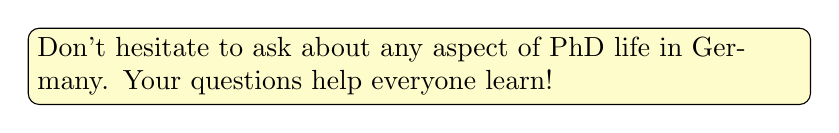
\begin{tikzpicture}
    \node[draw,rounded corners,fill=yellow!20,text width=0.8\textwidth] {
        Don't hesitate to ask about any aspect of PhD life in Germany. Your questions help everyone learn!
    };
\end{tikzpicture}

\vspace{1cm}

\alert{Contact Information}
\begin{itemize}
    \item Email: bijun.li@mpimet.mpg.de
    \item Twitter: @DrBijunLi
    \item LinkedIn: [Your LinkedIn Profile]
\end{itemize}
\end{frame}

\end{document}